\section{Das Java-Projekt}

F�r die grafische Darstellung und die Verwaltung der Programmzust�nde wurde das Java Spieleentwicklungs-Framework LibGDX\cite{LibGdx} verwendet. Das Projekt wurde mit IntelliJ idea entwickelt und nutzt in hohem Ma�e das gradle build system. Das IntelliJ projekt kann wie folgt importiert werden:

\lstinline{File -> import -> $project-root-folder -> build.gradle}

Das Projekt wurde mit \textbf{openjdk-1.8} entwickelt und l�sst sich am besten mit dieser Version von Java (Java 8) ausf�hren. Um das Projekt von Intellij Idea aus auszuf�hren, klicken Sie mit der rechten Maustaste auf die Klasse desktop/src/de.augsburg.hs.methoden.ki.DesktopLauncher und w�hlen Sie Run DektopLauncher.main. Die Verwendung von Intellij Idea ist nicht unbedingt erforderlich, jede Java-IDE, die \textbf{gradle unterst�tzt}, sollte ebenfalls funktionieren. 

Nach dem Start des Programms wird der folgende Screen angezeigt:

\begin{figure}[H]
    \centering
    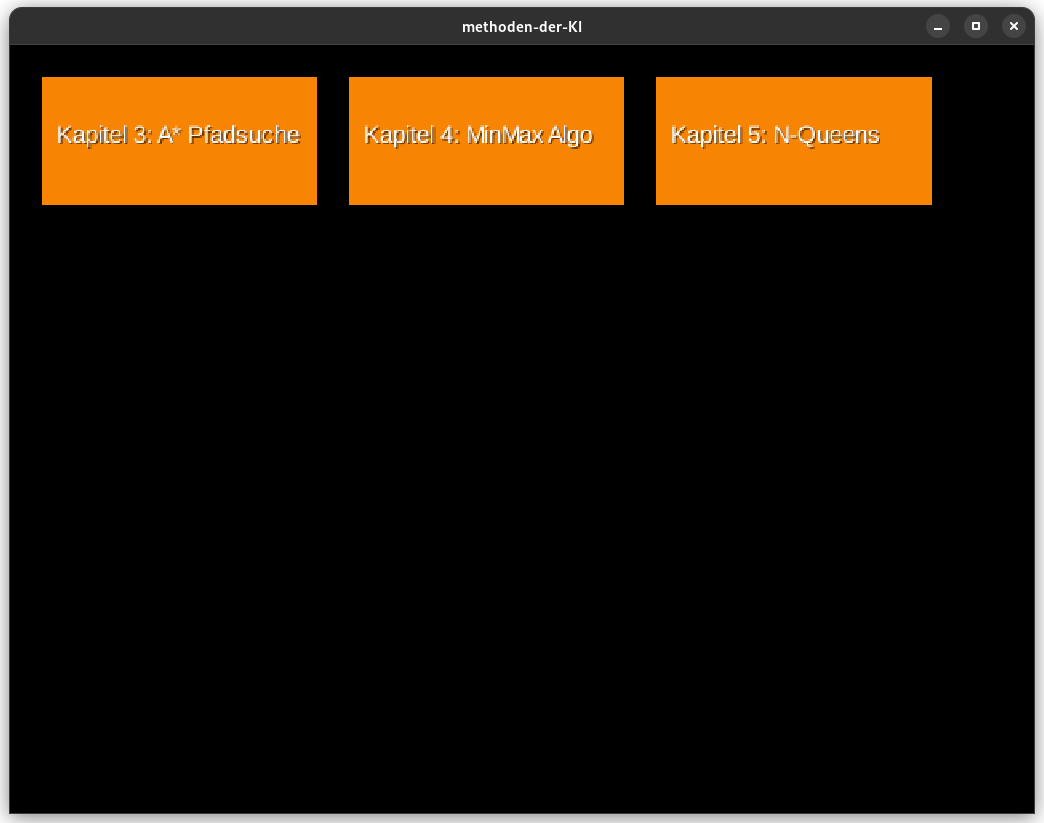
\includegraphics[width=0.6\textwidth]{figures/kap15/start-menu.png}
    \caption{Start Menu}
    \label{fig:start-menu-java}
\end{figure}

Durch Anklicken einer der Buttons wird der Benutzer zu dem entsprechenden Screen gef�hrt.